\documentclass{article}

% if you need to pass options to natbib, use, e.g.:
%     \PassOptionsToPackage{numbers, compress}{natbib}
% before loading neurips_2019

% ready for submission
% \usepackage{neurips_2019}

% to compile a preprint version, e.g., for submission to arXiv, add add the
% [preprint] option:
%     \usepackage[preprint]{neurips_2019}

% to compile a camera-ready version, add the [final] option, e.g.:
     \usepackage[final]{neurips_2019}

% to avoid loading the natbib package, add option nonatbib:
%     \usepackage[nonatbib]{neurips_2019}

\usepackage[utf8]{inputenc} % allow utf-8 input
\usepackage[T1]{fontenc}    % use 8-bit T1 fonts
\usepackage{hyperref}       % hyperlinks
\usepackage{url}            % simple URL typesetting
\usepackage{booktabs}       % professional-quality tables
\usepackage{amsfonts}       % blackboard math symbols
\usepackage{nicefrac}       % compact symbols for 1/2, etc.
\usepackage{microtype}      % microtypography
\usepackage{graphicx}       % display figure

\title{Project Proposal For 11-785}

% The \author macro works with any number of authors. There are two commands
% used to separate the names and addresses of multiple authors: \And and \AND.
%
% Using \And between authors leaves it to LaTeX to determine where to break the
% lines. Using \AND forces a line break at that point. So, if LaTeX puts 3 of 4
% authors names on the first line, and the last on the second line, try using

\author{%
  Ke Xu \\
  Electrical and Computing Engineering\\
  Carnegie Mellon University\\
  Pittsburgh, PA 15213 \\
  \texttt{kxu2@andrew.cmu.edu} \\

  \And
  Nicky Nocerino \\
  Electrical and Computing Engineering\\
  Carnegie Mellon University\\
  Pittsburgh, PA 15213 \\
  \texttt{nnocerin@andrew.cmu.edu} \\

  \And
  Yilin Wang \\
  Civil and Environment Engineering\\
  Carnegie Mellon University\\
  Pittsburgh, PA 15213 \\
  \texttt{yilinw2@andrew.cmu.edu} \\


  \And
  Zhufeng Fan \\
  Civil and Environment Engineering\\
  Carnegie Mellon University\\
  Pittsburgh, PA 15213 \\
  \texttt{zhufengf@andrew.cmu.edu} \\
  % examples of more authors
  % \And
  % Coauthor \\
  % Affiliation \\
  % Address \\
  % \texttt{email} \\
  % \AND
  % Coauthor \\
  % Affiliation \\
  % Address \\
  % \texttt{email} \\
  % \And
  % Coauthor \\
  % Affiliation \\
  % Address \\
  % \texttt{email} \\
  % \And
  % Coauthor \\
  % Affiliation \\
  % Address \\
  % \texttt{email} \\
}

\begin{document}

\maketitle

%%%%%%%%%%%%%%%%%%%%%%% Introduction %%%%%%%%%%%%%%%%%%%%
\section{Introduction}
The time series energy data are widely used right now. The data makes it possible to develop machine learning algorithms that can anaylyse and monitor the data collected and detect anomalous behaviour in the energy field, which contributes to improving the safety of the high power systems. The problem of finding patterns in data that do not conform to expected or normal behaviour is often referred to as Anomaly Detection. Since the mid-1990s, many computer science researchers have been working on how to automatically detect anomalies and many methods have been proposed. In particular, recently reserachers have successfully built some robust deep learning models with large dataset to detect anomalies. 

However, a significant amount of these approaches are based on supervised machine learning models that require (big) labelled datasets to be trained. Furthermore, some of the proposed methods do not consider the sequential nature of the data by assuming it is independent in time. To address the above issues, Joao Pereira and Margarida Silveira proposed a method called Variational Recurrent Autoencoders with Attention \cite{AuthorJM}, which uses time series data to train an unsupervised model. 

Our project is based on Joao Pereira and Margarida Silveira's work. First, we will implement their model and replicate their experimental results. Then we will try to improve the performance of the model by replacing Bi-LSTM with Transformer. Finally, we will implement a multi-class framework based on our previous model to discriminate between different anomalies using the latent features in the z-space.

%%%%%%%%%%%%%%%%%%%%%%% Literature Review %%%%%%%%%%%%%%%%%%%%
\section{Literature Review}
In recent years, various machine learning methods have been applied widely to automate the process monitoring and fault diagnosis. Artificial neural networks are popular due to a simplicity in logic and a powerful ability to deal with nonlinear problems such as abnormally detection. Typical supervised learning method with various build-in structures, for example, multi-layer perceptron (MLP) \cite{AuthorSI}, learning vector quantization networks (LVQ), were used to detect simple patterns such as shift, trend, cycle etc. With a further development of the network structure, hybrid model with a combination of models come into appear.

\subsection{Abnormally detection}
Abnormally detection has been widely used on system control and management. Potes and Cristhian development of an algorithm to classify normal/abnormal heart sounds from the observation dataset on human bodies. A total of 124 time-frequency features were extracted from the phonocardiogram (PCG) which is used as an input of a convolutional neural network (CNN) based on an ensemble of classifiers combining the outputs of AdaBoost. \cite{AuthorPotes} Du and Min (2017), proposed a Long Short-Term
Memory (LSTM), to model a system log as a natural language sequence. With and automatic learning from log patterns, it allowed the algorithm to detect anomalies when log patterns deviate from the model trained from log data under normal execution. \cite{AuthorDu}

\subsection{Auto-encoder (AE) and Auto-decoder (AD) network}
With addressing a large scale of data and high-dimensional level of learning, autoencoder (AE) makes its way into health monitoring \cite{AuthorRZ}, fault diagnosis AE models could learn representative features from raw data by reconstructing input data from an artificial corruption. For years, AE models have been widely used on diverse fields to deal with the practical problem. Chen, Min, et al (2017), proposes a convolutional autoencoder deep learning framework to support unsupervised image
features learning for lung module with a small amount of labeled data for efficient feature learning. Kamper and Herman (2015), proposed an unsupervised neural network feature extractor without resources in zero-resource settings. They achieved a two-third of relative improvement with the feature extractor in a word discrimination task. \cite{AuthorKa} Fan and Cheng (2018) investigates the potential of autoencoders in detecting anomalies in building energy data. Specific methods have been
designed to evaluate the autoencoder performance, the results can be used as foundation for building professionals to develop advanced tools for anomaly detection. 

\begin{figure}[!t]
    \centering
    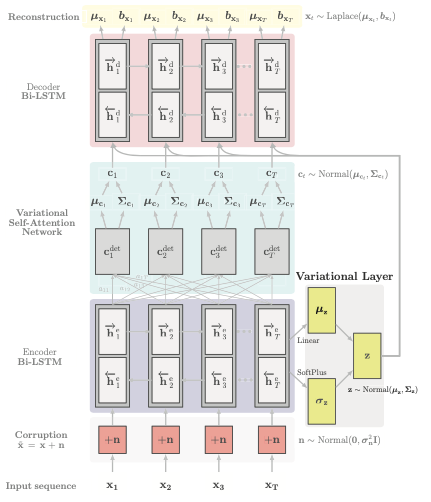
\includegraphics[width=0.7\textwidth]{images/BiLSTM.png}
    \caption{Variational Bi-LSTM Autoencoder with Variational Self-Attention.}
\end{figure}
%%%%%%%%%%%%%%%%%%%%%%% Model Baseline %%%%%%%%%%%%%%%%%%%%
\section{Model Baseline}
The original model for this paper is composed of 2 parts, a Variational Bi-LSTM autoencoder and an Anomaly detection strategy, and operate on a data set composed of N independent sequences, split into T timesteps with $d_{xn}$ dimensional features. Figure 1 illustrates the proposed model.

The Variational Bi-LSTM autoencoder takes in a sequence of observations, adds noises of Normal(0, $\sigma_{n}^2$) and is trained to return a  clean version of the data (noise is only applied during training). The encoder is parameterized by using a bi-LSTM with tanh activations and a hidden layer in both the forwards and backwards directions. Furthermore, an attention mechanism is integrated called a Variational Self Attention Mechanism (VSAM) to create a context vector which is normalized over
the seconds dimension. The decoder is also a Bi-LSTM with tanh activations that at each timestep receives a latent representation and a context vector and uses a Laplace Distribution in order to minimize the $L_1$ reconstruction loss.

The anomaly detection is based on the principle that the auto-encoder will be trained on normal sequences and will learn the normal pattern of behaviour. Meaning that normal sequences will be well reconstructed whereas anomalous ones will not. The reconstruction probability is calculated and is used to determine whether a sequence is anomalous. 

%%%%%%%%%%%%%%%%%%%%%%% Dataset Description %%%%%%%%%%%%%%%%%%%%
\section{Dataset Description}
We have not finally decided what data to use. But here are two candidates:

\subsection{EMHIRES dataset}
EMHIRES is the first publically available European solar power generation dataset derived from meteorological sources that is available up to NUTS-2 level. It was generated applying the PVGIS model to capture local geographical information to generate meteorologically derived solar power time series at high temporal and spatial resolution. This allows for a better understanding of the solar resource at the precise location of wind farms.

EMHIRES provides RES-E generation time series for the EU-28 and neighbouring countries. The solar power time series are released at hourly granularity and at different aggregation levels: by country, power market bidding zone, and by the European Nomenclature of territorial units for statistics (NUTS) defined by EUROSTAT; in particular, by NUTS 1 and NUTS 2 level. The time series provided by bidding zones include special aggregations to reflect the power market reality where this deviates from political or territorial boundaries.

The overall scope of EMHIRES is to allow users to assess the impact of meteorological and climate variability on the generation of solar power in Europe and not to mime the actual evolution of solar power production in the latest decades. For this reason, the hourly solar power generation time series are released for meteorological conditions of the years 1986-2015 (30 years) without considering any changes in the solar installed capacity. Both the Country level and NTUS level data contain 262,968 hourly time steps, from 1986/1/1 00:00 to 2015/12/31 23:00.

\begin{table}
  \caption{Raw inspection data records count by inspection year}
  \label{obd data}
  \centering
  \begin{tabular}{cccc}
    \toprule
    \multicolumn{4}{c}{Samples}                   \\
    \cmidrule(r){1-4}
    Year & Records & Year & Records      \\
    \midrule
    2000 & $3,000,804$ & 2003 & $3,151,591$     \\
    2001 & $3,057,150$ & 2004 & $5,562,887$       \\
    2002 & $3,103,306$ & 2005 & $5,611,680$      \\
    \bottomrule
  \end{tabular}
\end{table}

\subsection{OBD dataset}
The OBD dataset is bulit on the Pennsylvania On Board Diagnostics emission test data provided by the state Department of Transportation. Pennsylvania has a decentralized inspection program that requires annual safety inspections for all vehicles in all counties, in addition to annual emissions inspections in a subset of counties with air quality non-attainment issues for mostly near urban areas. This is a very long time series inspection records data from 2000 to 2016. Table 1 shows a summary of all raw records by year.

There are 132 variables in the dataset, each unique record contains:
\begin{itemize}

\item Inspection time
    
\item Vehicle characteristics information, such as VIN, fuel type, odometer reading, etc.

\item OBD data, such as OBD systems readiness status, Diagnostic Trouble status, Dilution Correctness status, etc.

\end{itemize}


%%%%%%%%%%%%%%%%%%%%%%% Methods %%%%%%%%%%%%%%%%%%%%
\section{Methods}
The primary method expansion for this project will be the replacement of the Variational Bi-LSTM autoencoder with an entirely attention based Transformer model \cite{NIPS2017_7181}. We believe this model will be more capable of encoding normal data, which should improve our ability to detect anomalies.


{
\bibliographystyle{unsrt}
\bibliography{egbib}
}

\end{document}
